\documentclass{beamer}

% For more themes, color themes and font themes, see:
% http://deic.uab.es/~iblanes/beamer_gallery/index_by_theme.html
%
\mode<presentation>
{
  %\usetheme{Frankfurt}       % or try default, Darmstadt, Warsaw, ...
  %\usetheme{Malmoe}
  \usetheme{Madrid}
  \usecolortheme{default} % or try albatross, beaver, crane, ...
  \usefonttheme{serif}    % or try default, structurebold, ...
  \setbeamertemplate{navigation symbols}{}
  \setbeamertemplate{caption}[numbered]
} 

\usepackage[brazil,portuguese]{babel}
\usepackage[utf8x]{inputenc}
\usepackage{chemfig}
\usepackage[version=3]{mhchem}
\usepackage{wrapfig}
\usepackage[caption = false]{subfig}
\usepackage{floatflt,graphicx}
% On Overleaf, these lines give you sharper preview images.
% You might want to `comment them out before you export, though.
\usepackage{pgfpages}
\pgfpagesuselayout{resize to}[%
  physical paper width=8in, physical paper height=6in]

\makeatletter
\long\def\beamer@author[#1]#2{%
  \def\insertauthor{\def\inst{\beamer@insttitle}\def\and{\beamer@andtitle}%
  \begin{tabular}{l}#2\end{tabular}}%
  \def\beamer@shortauthor{#1}%
  \ifbeamer@autopdfinfo%
    \def\beamer@andstripped{}%
    \beamer@stripands#1 \and\relax
    {\let\inst=\@gobble\let\thanks=\@gobble\def\and{, }\hypersetup{pdfauthor={\beamer@andstripped}}}
  \fi%
}
\makeatother
\setbeamertemplate{caption}{\raggedright\insertcaption\par}
  
% Here's where the presentation starts, with the info for the title slide
\institute{Universidade Técnológica Federal do Paraná - Campus Pato Branco\\Departamento Acadêmico de Informática\\Curso de Engenharia de Computação}
\title{Consultas por similaridade em bases de dados complexos utilizando técnica OMNI em SGBDR}
\subtitle{Trabalho de Conclusão de Curso}
\author{
Aluno: Cristiano José Mendes Matsui\\
Orientador: Dr. Ives Renê Venturini Pola\\
Coorientadora: Dra. Fernanda Paula Barbosa Pola
}
\date{\today}

\begin{document}

\captionsetup[subfigure]{labelformat=empty}

\begin{frame}[plain]
     \vfill
     \centering

     \begin{beamercolorbox}[sep=8pt,center,colsep=-4bp,rounded=true,shadow=true]{institute}
        \usebeamerfont{institute}\insertinstitute
     \end{beamercolorbox}

     {\usebeamercolor[fg]{titlegraphic}\inserttitlegraphic\par}

     \begin{beamercolorbox}[sep=8pt,center,colsep=-4bp,rounded=true,shadow=true]{title}
        \usebeamerfont{title}\inserttitle\par%
        \ifx\insertsubtitle\@empty%
        \else%
        \vskip0.25em%
        {\usebeamerfont{subtitle}\usebeamercolor[fg]{subtitle}\insertsubtitle\par}%
      \fi%     
     \end{beamercolorbox}%

     \vskip1em\par

     \begin{beamercolorbox}[sep=8pt,center,colsep=-4bp,rounded=true,shadow=true]{author}
        \usebeamerfont{author}\insertauthor
     \end{beamercolorbox}

     \begin{beamercolorbox}[sep=8pt,center,colsep=-4bp,rounded=true,shadow=true]{date}
        \usebeamerfont{date}\insertdate
     \end{beamercolorbox}\vskip0.5em

    \end{frame}
\author{Cristiano Matsui}
\institute{UTFPR}
\title{Trabalho de Conclusão de Curso}
% These three lines create an automatically generated table of contents.
\begin{frame}{Sumário}
  \tableofcontents
\end{frame}

\section{Introdução}

\begin{frame}{Introdução}
  \begin{itemize}
    \item Crescimento do uso de dados multimídia
      \begin{itemize}
	\item Imagens, vídeos, áudio...\newline
      \end{itemize}
    \item ``dados comuns'' x ``dados complexos''\newline
	\begin{figure}[H]
			\centering
			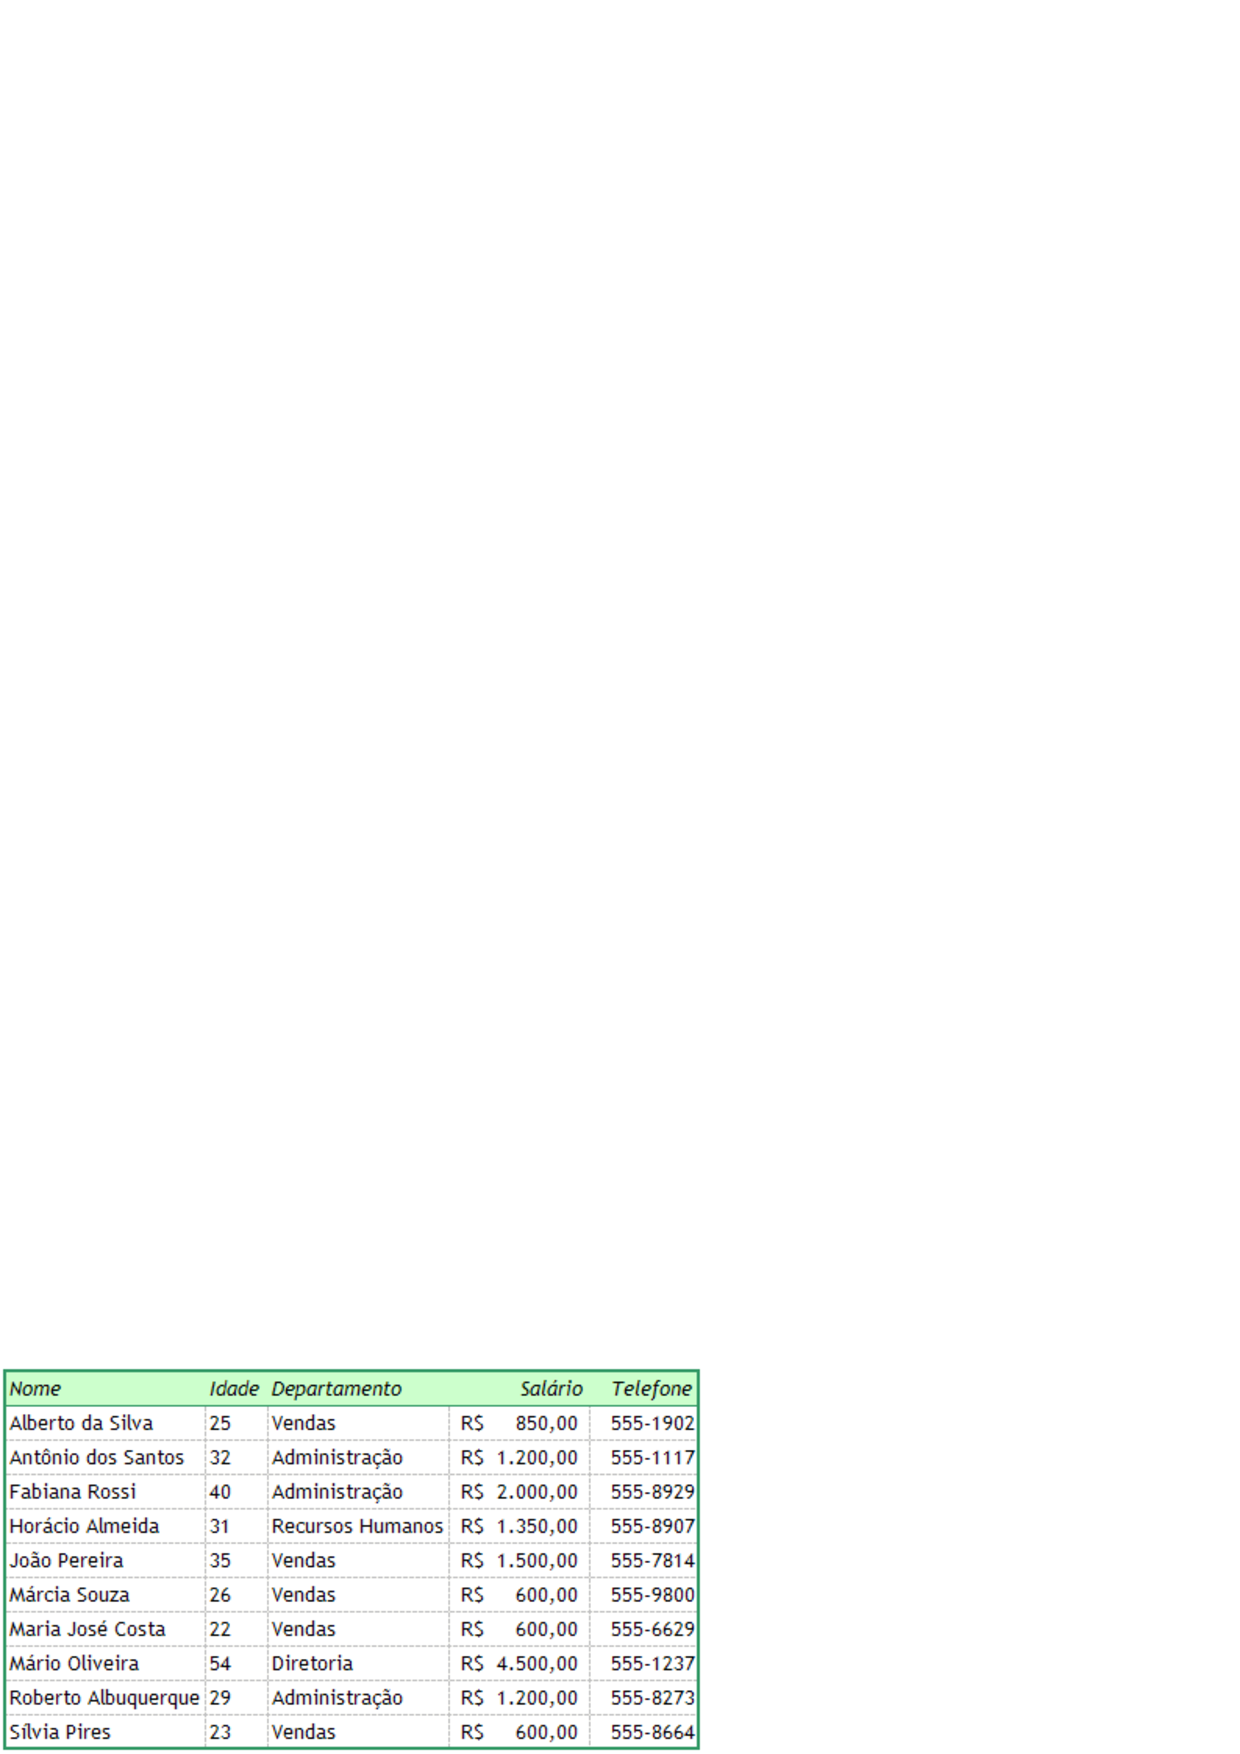
\includegraphics[width=.5\textwidth]{dado_comum.png}
			\label{fig:dado_comum}
	\end{figure}
    \item Novos operadores de consulta\newline
  \end{itemize}


\end{frame}

\begin{frame}{Introdução}
  \begin{itemize}
   \item Consultas por similaridade\newline
      \begin{itemize}
	  \item Consulta por abrangência (\textit{Range query})\newline
	  \item Consulta aos k-vizinhos mais próximos (\textit{k-Nearest Neighbors query})
      \end{itemize}
	
	\begin{figure}
\centering
\begin{minipage}{.4\textwidth}
  \centering
  \includegraphics[width=.9\linewidth]{rq.png}
  \caption{\textit{Range query}}
  \label{fig:rq}
\end{minipage}%
\begin{minipage}{.6\textwidth}
  \centering
  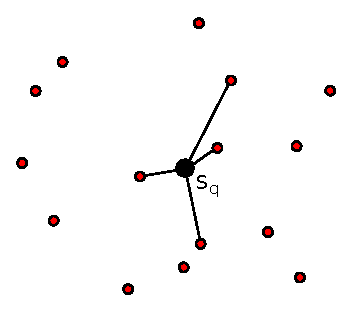
\includegraphics[width=.6\linewidth]{knnq.eps}
  \caption{\textit{kNN query}}
  \label{fig:knnq}
\end{minipage}
\end{figure}
	
  \end{itemize}


\end{frame}

\begin{frame}{Introdução}

  \begin{itemize}
   \item Consultas por similaridade são custosas\newline
   
   \begin{itemize}
      \item Complexidade dos dados\newline
      \item Tamanho da base\newline
   \end{itemize}
   
   \item Torna-se necessário otimizar estes procedimentos\newline
   
   \item Uso da técnica OMNI
  \end{itemize}

 
\end{frame}

\section{Objetivos}

\begin{frame}{Objetivos}
  \begin{itemize}
   \item Objetivos Gerais
   \begin{itemize}
      \item Consultas por similaridade utilizando OMNI em SGBDR\newline
   \end{itemize}
   \item Objetivos Específicos
   \begin{itemize}
      \item Modelagem;
      \item Extrair características;
      \item Inserção das características no banco;
      \item Criação das estruturas OMNI;
      \item Analisar e comparar os resultados obtidos.
   \end{itemize}
   
  \end{itemize}

\end{frame}

\section{Técnica OMNI}

\begin{frame}{Técnica OMNI}

  \begin{itemize}
   \item Reduz o número de cálculos de distância desnecessários\newline
   
   \item Uso de uma base de focos\newline
   
   \item \textit{minimum bounding OMNI region - mbOr}\newline
   
   \item Desigualdade triangular e conceito de bola fechada

  \end{itemize}

 
\end{frame}


\begin{frame}{Técnica OMNI}

	\begin{figure}
	    \centering
	    \begin{minipage}{.5\textwidth}
	      \centering
	      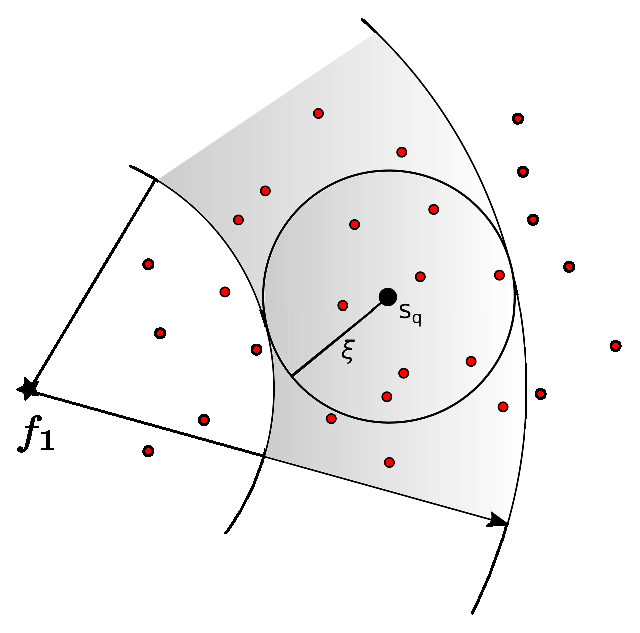
\includegraphics[width=.9\linewidth]{rg_omni_1.eps}


	    \end{minipage}%
	    \begin{minipage}{.5\textwidth}
	      \centering
	      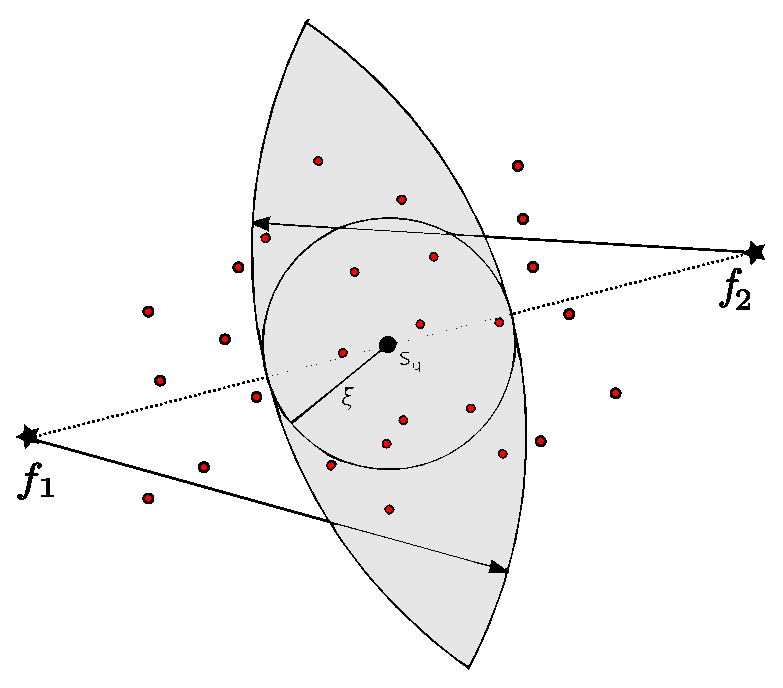
\includegraphics[width=.95\linewidth]{rg_omni_2.eps}


	    \end{minipage}
	\end{figure}
 
\end{frame}


\begin{frame}{Técnica OMNI}
    \begin{columns}
      \begin{column}{0.6\linewidth}
	\begin{itemize}
	 \item minimum bounding OMNI region\newline
	    \begin{itemize}
	      \item Desigualdade triangular\newline
		\begin{itemize}
		  \item $d_{f}(s_i) \leq d_{f}(s_q) + d(s_i, s_q)$\newline
		  
		  \item $d(s_i, s_q) \geq |d_{f}(s_i) - d_{f}(s_q)|$\newline
		\end{itemize}
	      \item Conceito de bola\newline
		\begin{itemize}
		  \item $d(s_i, s_q) \leq \xi$\newline
		\end{itemize}
	    \end{itemize}
	\item $\xi \geq d(s_i,s_q) \geq |d_f(s_i) - d_f(s_q)|$\newline
	\end{itemize}
      \end{column}
%       \hfill
      \begin{column}{0.4\linewidth}
	    \begin{figure}[H!]
% 			\hspace{4.0cm}
% 			\centering
	      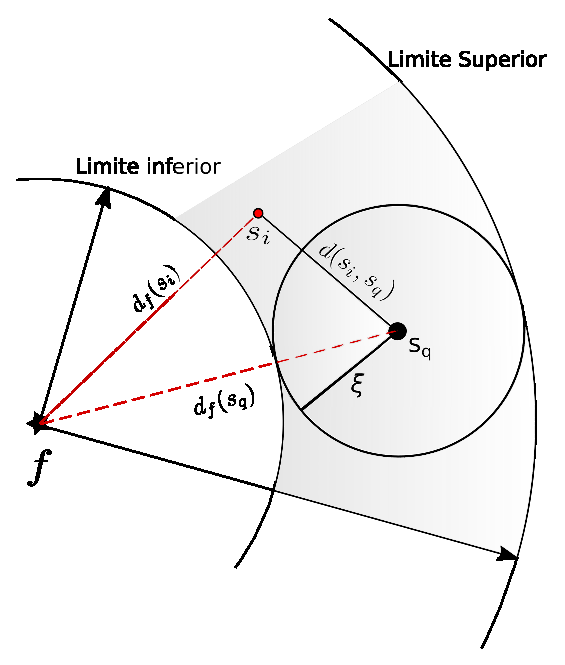
\includegraphics[width=1\linewidth]{destri_omni.eps}
	    \end{figure}
      \end{column}

  \end{columns}
  \begin{itemize}
   \item $|d_f(s_i) - d_f(s_q)| \leq \xi$ $\leftarrow$ Equação de pertinência à \textit{mbOr}
  \end{itemize}

\end{frame}

\begin{frame}{Técnica OMNI}
	\begin{itemize}
	 \item $|d_f(s_i) - d_f(s_q)| \leq \xi$ $\leftarrow$ Equação de pertinência à \textit{mbOr}\newline
	 \item $|d_f(s_4) - d_f(s_q)| < \xi$\newline
	 \item Pertence à \textit{mbOr}!
	\end{itemize}

	\begin{figure}[H]
			\centering
			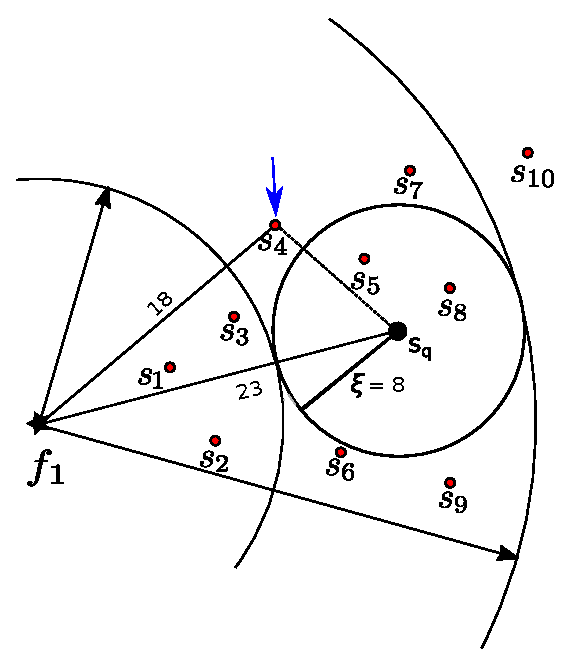
\includegraphics[width=.35\textwidth]{dados/figuras/rg_ex4.eps}
	\end{figure} 

\end{frame}

\begin{frame}{Técnica OMNI}
	\begin{itemize}
	 \item $|d_f(s_i) - d_f(s_q)| \leq \xi$ $\leftarrow$ Equação de pertinência à \textit{mbOr}\newline
	 \item $|d_f(s_3) - d_f(s_q)| > \xi$\newline
	 \item Não pertence à \textit{mbOr}!
	\end{itemize}

	\begin{figure}[H]
			\centering
			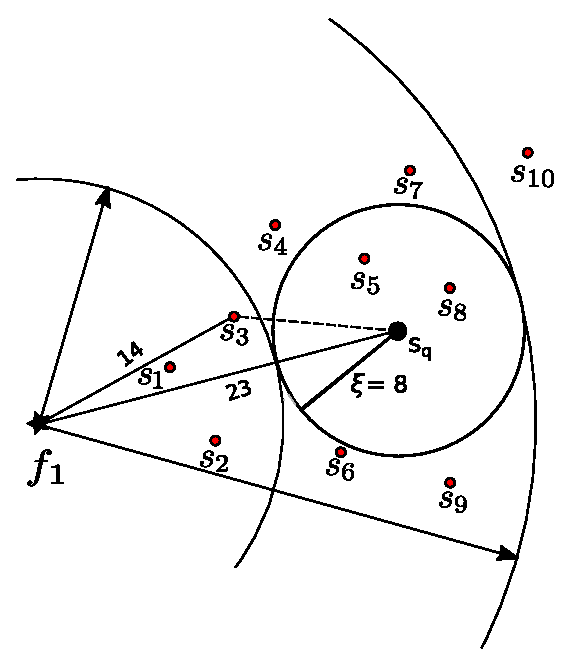
\includegraphics[width=.35\textwidth]{rg_ex2.eps}
	\end{figure}

\end{frame}

\begin{frame}{Técnica OMNI}
  
  \begin{itemize}
   \item Escolha dos focos\newline  
   \item Número ótimo de focos
      \begin{itemize}
	\item \textit{Box counting}\newline
	    \begin{itemize}
		\item ($\lceil D \rceil +1$) \newline
	    \end{itemize}
	\item Gráfico de podas $\times$ número de focos\newline
      \end{itemize}
   	
  \end{itemize}

\begin{figure}[H]
    \centering
    \includegraphics[width=.45\textwidth]{dados/figuras/focoHC.eps}
\end{figure}
 
\end{frame}

\section{Bases de Dados}

\begin{frame}{Bases de Dados}
  \begin{itemize}
   \item Duas bases de dados utilizadas\newline
  \item CAT\_DOG - 25000 imagens
      \begin{itemize}
       \item Imagens de cães e gatos
       \item Características extraídas via Python + Scikit-Image
	  \begin{itemize}
	    \item Cor - Histograma
	    \item Textura - dissimilaridade, contraste, correlação
	    \item Forma - área, excentricidade, área convexa\newline
	  \end{itemize}
      \end{itemize}

  \item HC - 500000 imagens
      \begin{itemize}
	\item Características de imagens médicas já extraídas
	\item Histograma de 256 tons de cinza
      \end{itemize}
      
  \end{itemize}

\end{frame}

\begin{frame}{Bases de Dados}
  \begin{itemize}
   \item Modelagem CAT\_DOG
  \end{itemize}
  \begin{figure}[H]
      \centering
      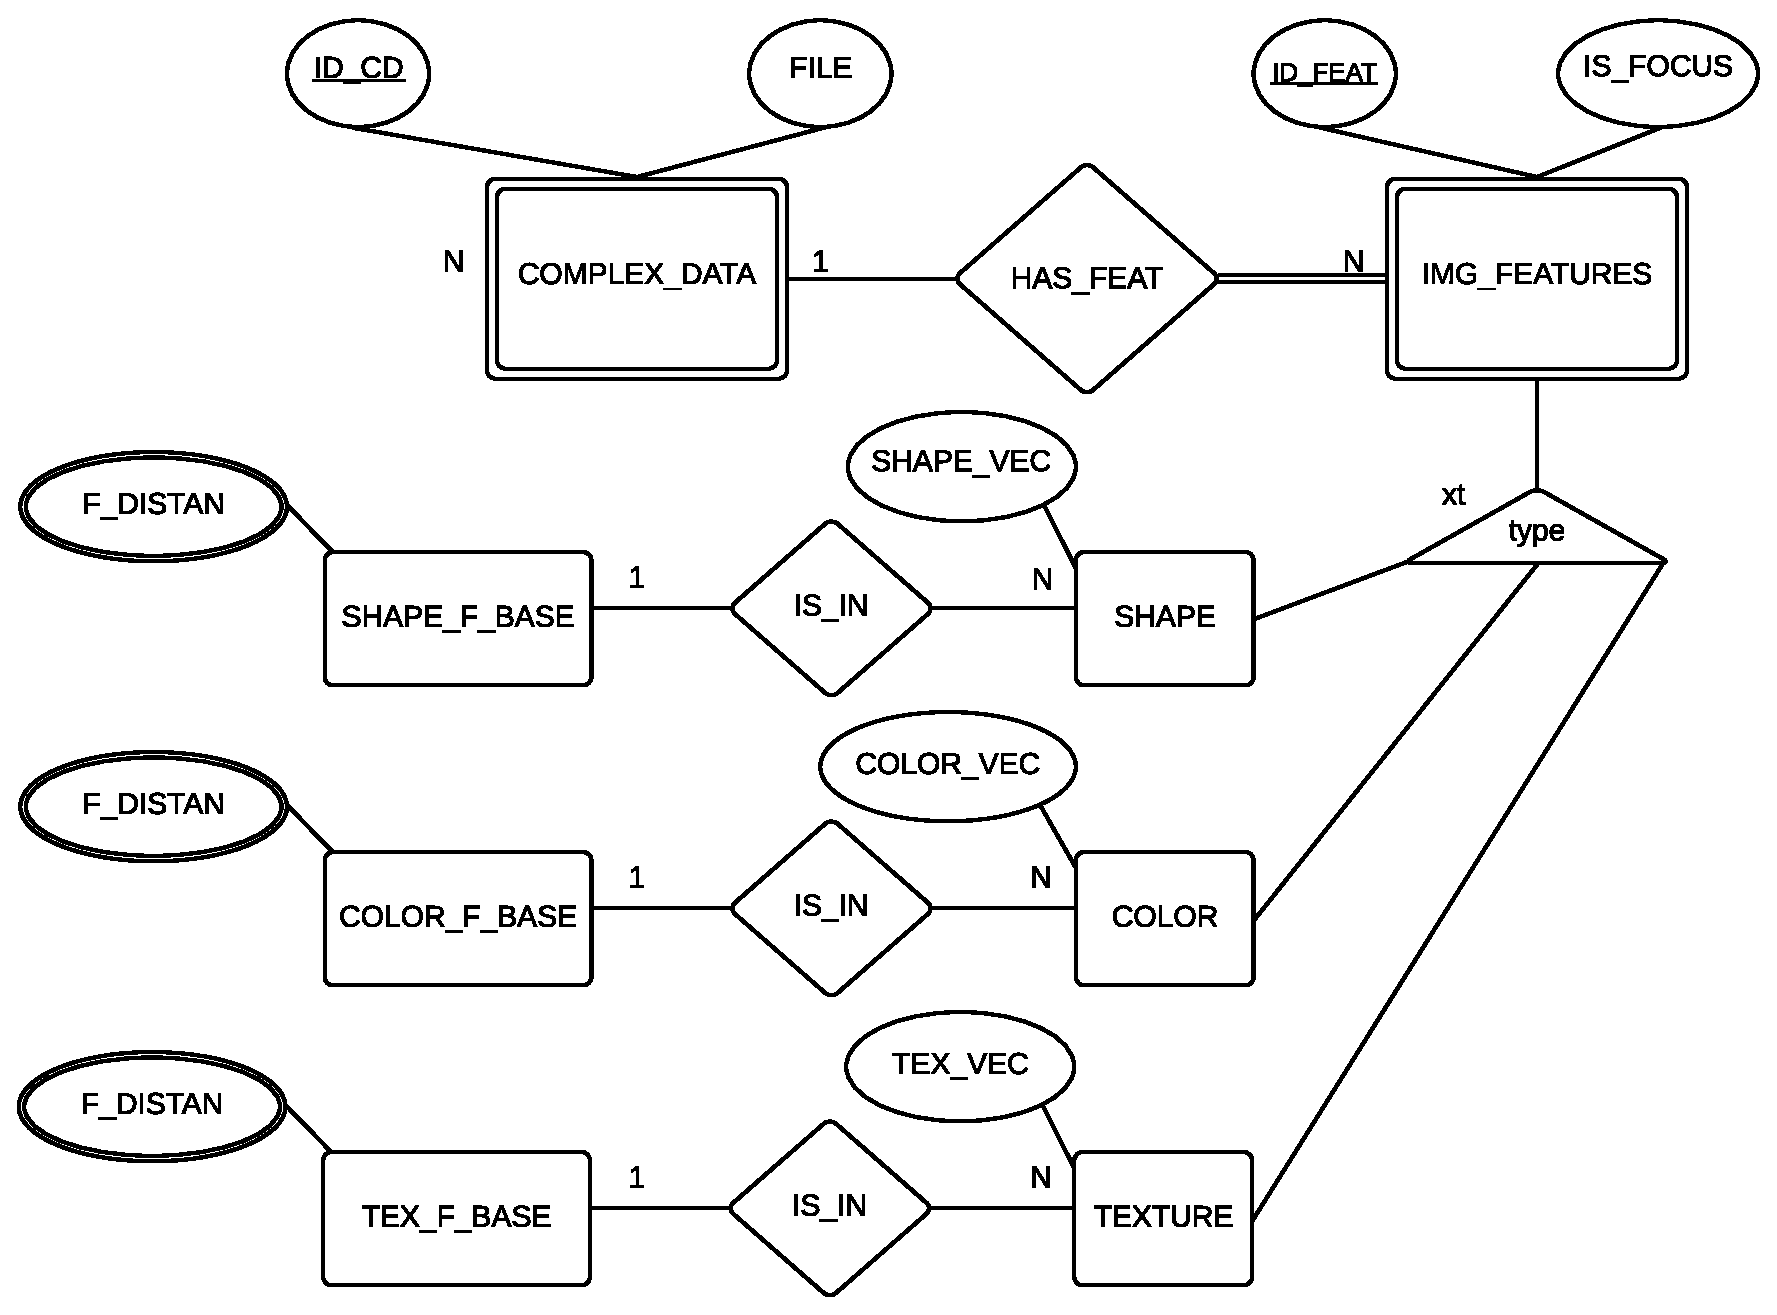
\includegraphics[width=.7\textwidth]{dados/figuras/mer_cd.eps}
  \end{figure}
\end{frame}

\begin{frame}{Bases de Dados}
  \begin{itemize}
   \item Modelagem HC
  \end{itemize}
  \begin{figure}[H]
      \centering
      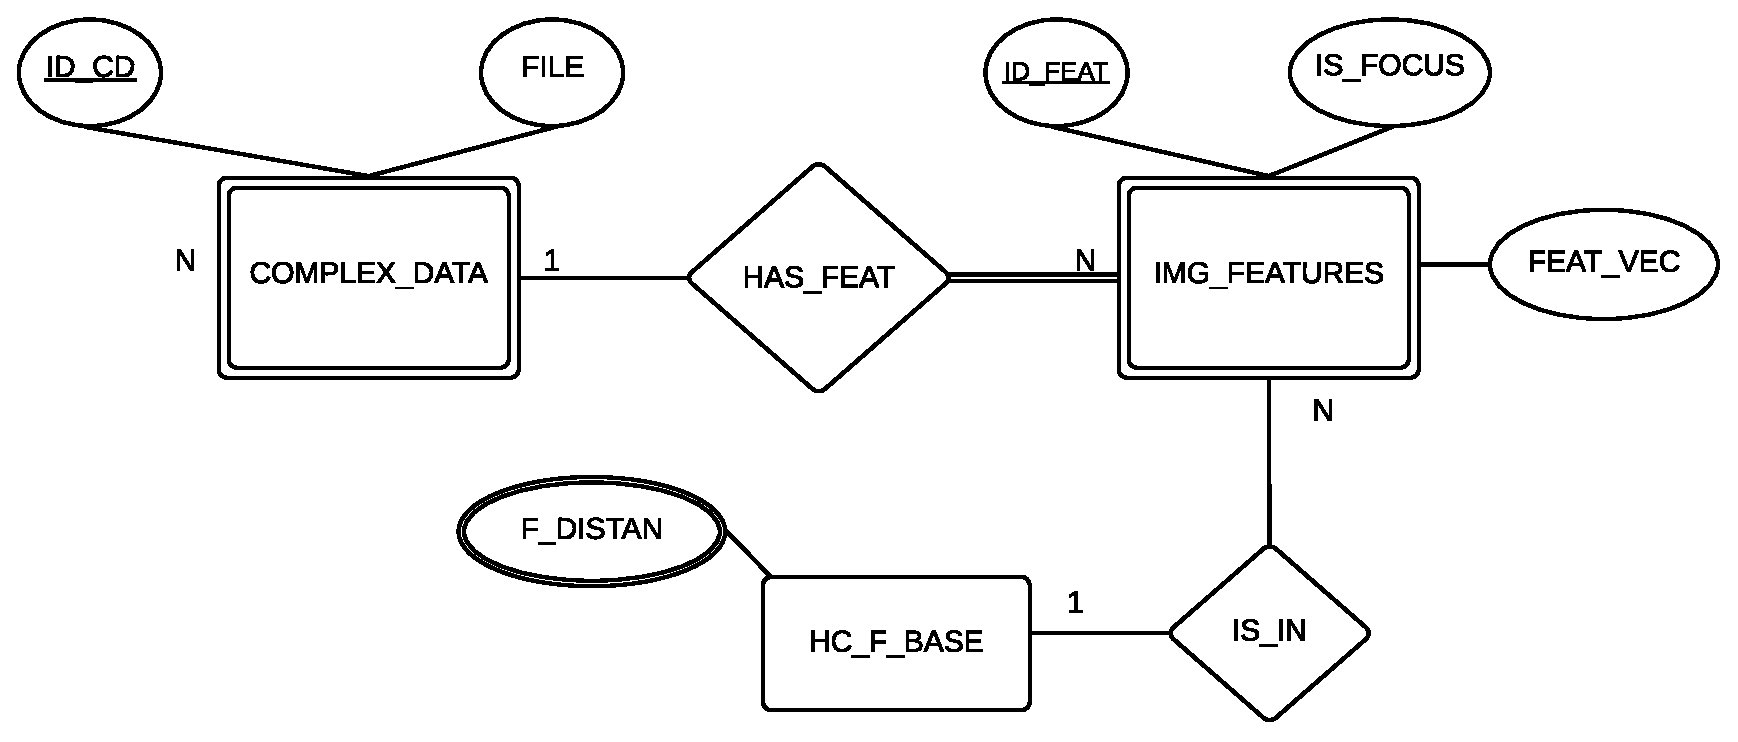
\includegraphics[width=.9\textwidth]{dados/figuras/mer_hc.eps}
  \end{figure}
\end{frame}

\section{Resultados do Trabalho}

\begin{frame}{Resultados do Trabalho}
  \begin{itemize}
   \item Testes realizados utilizando distâncias $L_1$, $L_2$ e $L_\infty$\newline
   \item Média de 10 medições distintas para um mesmo centro\newline
   \item Sequencial e OMNI com números distintos de focos\newline
   \item Utilização das estruturas de indexação\newline
  \end{itemize}
\end{frame}

\begin{frame}{Resultados do Trabalho}
 \begin{itemize}
  \item Base CAT\_DOG - Consulta por abrangência - $L_1$ - FORMA
 \end{itemize}
  
  \begin{table}[H]
    \centering
   \begin{tabular}{l c c c}
%         \toprule
            &Tempo de Execução(ms)&Nº Podas de Cálculos\\ \hline
%         \midrule
            Sequencial & 8,721 & - \\
            \textbf{OMNI 1 Foco} & \textbf{1,747} & 24935 \\
            OMNI 2 Focos & 5,201 & 24935 \\
            OMNI 3 Focos & 7,606 & 24935 \\
            OMNI 4 Focos & 10,107 & 24935 \\
            OMNI 5 Focos & 12,271 & 24935 \\ \hline
%         \bottomrule
    \end{tabular}
\end{table}
  
\end{frame}

\begin{frame}{Resultados do Trabalho}
 \begin{itemize}
  \item Base CAT\_DOG - Consulta por abrangência - $L_2$ - FORMA
 \end{itemize}
  
  \begin{table}[H]
    \centering
   \begin{tabular}{l c c c}
%         \toprule
            &Tempo de Execução(ms)&Nº Podas de Cálculos\\ \hline
%         \midrule
            Sequencial & 8,728 & - \\
            \textbf{OMNI 1 Foco} & \textbf{1,825} & 24935 \\
            OMNI 2 Focos & 4,988 & 24935 \\
            OMNI 3 Focos & 7,525 & 24935 \\
            OMNI 4 Focos & 8,994 & 24935 \\
            OMNI 5 Focos & 11,591 & 24935 \\ \hline
    \end{tabular}
\end{table}
  
\end{frame}

\begin{frame}{Resultados do Trabalho}
 \begin{itemize}
  \item Base CAT\_DOG - Consulta por abrangência - $L_\infty$ - FORMA
 \end{itemize}
  
  \begin{table}[H]
    \centering
   \begin{tabular}{l c c c}
%         \toprule
            &Tempo de Execução(ms)&Nº Podas de Cálculos\\ \hline
%         \midrule
            Sequencial & 8,805 & - \\
            \textbf{OMNI 1 Foco} & \textbf{2,051} & 24935 \\
            OMNI 2 Focos & 4,638 & 24935 \\
            OMNI 3 Focos & 8,563 & 24935 \\
            OMNI 4 Focos & 9,651 & 24935 \\
            OMNI 5 Focos & 11,626 & 24935 \\ \hline
    \end{tabular}
\end{table}
  
\end{frame}

\begin{frame}{Resultados do Trabalho}
 \begin{itemize}
  \item Base CAT\_DOG - Consulta por abrangência - $L_1$ - TEXTURA
 \end{itemize}
  
  \begin{table}[H]
    \centering
   \begin{tabular}{l c c c}
%         \toprule
            &Tempo de Execução(ms)&Nº Podas de Cálculos\\ \hline
%         \midrule
            Sequencial & 8,710 & - \\
            \textbf{OMNI 1 Foco} & \textbf{1,531} & 24950 \\
            OMNI 2 Focos & 4,512 & 24950 \\
            OMNI 3 Focos & 6,838 & 24950 \\
            OMNI 4 Focos & 9,447 & 24950 \\
            OMNI 5 Focos & 11,182 & 24950 \\ \hline
    \end{tabular}
\end{table}
  
\end{frame}

\begin{frame}{Resultados do Trabalho}
 \begin{itemize}
  \item Base CAT\_DOG - Consulta por abrangência - $L_1$ - COR
 \end{itemize}
  
  \begin{table}[H]
    \centering
   \begin{tabular}{l c c c}
%         \toprule
            &Tempo de Execução(ms)&Nº Podas de Cálculos\\ \hline
%         \midrule
            Sequencial & 8,334 & - \\
            \textbf{OMNI 1 Foco} & \textbf{1,675} & 24923 \\
            OMNI 2 Focos & 4,819 & 24923 \\
            OMNI 3 Focos & 8,073 & 24923 \\
            OMNI 4 Focos & 9,628 & 24923 \\
            OMNI 5 Focos & 12,925 & 24923 \\ \hline
    \end{tabular}
\end{table}
  
\end{frame}

\begin{frame}{Resultados do Trabalho}
 \begin{itemize}
  \item Base HC - Consulta por abrangência - $L_1$
 \end{itemize}
  
  \begin{table}[H]
    \centering
   \begin{tabular}{l c c c}
%         \toprule
            &Tempo de Execução(ms)&Nº Podas de Cálculos\\ \hline
%         \midrule
            Sequencial & 4566,851 & - \\
            OMNI 1 Foco & 448,105 & 484381 \\
            \textbf{OMNI 2 Focos} & \textbf{292,709} & 490599 \\
            OMNI 3 Focos & 361,712& 499406 \\
            OMNI 4 Focos & 462,795 & 499845 \\
            OMNI 5 Focos & 882,159 & 499937 \\ \hline
    \end{tabular}
\end{table}
  
\end{frame}

\begin{frame}{Resultados do Trabalho}
 \begin{itemize}
  \item Base HC - Consulta por abrangência - $L_2$
 \end{itemize}
  
  \begin{table}[H]
    \centering
   \begin{tabular}{l c c c}
%         \toprule
            &Tempo de Execução(ms)&Nº Podas de Cálculos\\ \hline
%         \midrule
            Sequencial & 4310,409 & - \\
            OMNI 1 Foco & 1215,435 & 422246 \\
            \textbf{OMNI 2 Focos} & \textbf{307,757} & 484381 \\
            OMNI 3 Focos & 556,683 & 485574 \\
            OMNI 4 Focos & 598,664 & 488229 \\
            OMNI 5 Focos & 952,008 & 488841 \\ \hline
    \end{tabular}
\end{table}
  
\end{frame}

\begin{frame}{Resultados do Trabalho}
 \begin{itemize}
  \item Base HC - Consulta por k-vizinhos mais próximos - $L_2$
 \end{itemize}
  
  \begin{table}[H]
    \centering
   \begin{tabular}{l c c}
%         \toprule
            &Tempo de Execução(ms)\\ \hline
%         \midrule
            \textbf{Sequencial} & \textbf{4733,579}  \\
            OMNI 1 Foco & 6519,995  \\
            OMNI 2 Focos & 6341,987  \\
            OMNI 3 Focos & 7490,256 \\
            OMNI 4 Focos & 7548,550 \\
            OMNI 5 Focos & 10348,541 \\ \hline
    \end{tabular}
\end{table}
  
\end{frame}

\begin{frame}{Resultados do Trabalho}
 \begin{itemize}
  \item Ganho de Performance - GP
  \item $GP_\% = (T_o/T_s - 1)*100$
 \end{itemize}

 \begin{table}[!htb]
    \begin{minipage}{.5\linewidth}
      \caption{}
      \centering
      \begin{tabular}{l c}
%         \toprule
            CAT\_DOG&GP (\%)\\ \hline
%         \midrule
            L$_1$ - FORMA & 399,20 \\
            L$_2$ - FORMA & 378,24 \\
            L$_\infty$ - FORMA & 329,30 \\
            L$_1$ - TEXTURA & 468,91 \\
            L$_1$ - COR & 397,55 \\ \hline
%         \bottomrule
    \end{tabular}
    \end{minipage}%
    \begin{minipage}{.5\linewidth}
      \centering
        \caption{}
   \begin{tabular}{l c}
%         \toprule
            HC&GP (\%)\\ \hline
%         \midrule
            L$_1$ & 1460,20 \\
            L$_2$ & 1304,04 \\
            L$_\infty$ & - \\ \hline
%         \bottomrule
    \end{tabular}
    \end{minipage} 
\end{table}
 

 
\end{frame}

% 
% \begin{frame}{Resultados}
%  \begin{itemize}
%   \item Consulta por similaridade - FORMA
%  \end{itemize}
% \begin{figure}[H]
%   \centering
%   \subfloat[cat.50 - $S_q$]{\includegraphics[width=.20\textwidth]{dados/figuras/cat50.jpg}} \hspace{2cm}
%   \subfloat[cat.9211]{\includegraphics[width=.20\textwidth]{dados/figuras/cat9211.jpg}} \hspace{2cm}
%   \subfloat[dog.10089]{\includegraphics[width=.20\textwidth]{dados/figuras/dog10089.jpg}}\\
%   \subfloat[dog.3125]{\includegraphics[width=.20\textwidth]{dados/figuras/dog3125.jpg}} \hspace{2cm}
%   \subfloat[cat.5010]{\includegraphics[width=.20\textwidth]{dados/figuras/cat5010.jpg}} \hspace{2cm}
%   \subfloat[cat.4258]{\includegraphics[width=.20\textwidth]{dados/figuras/cat4258.jpg}} \\
% \end{figure}
% \end{frame}
% 
% \begin{frame}{Resultados}
%  \begin{itemize}
%   \item Consulta por similaridade - TEXTURA
%  \end{itemize}
% \begin{figure}[H]
%   \centering
%   \subfloat[dog.6431 - $S_q$]{\includegraphics[width=.20\textwidth]{dados/figuras/dog6431.jpg}} \hspace{2cm}
%   \subfloat[cat.3864]{\includegraphics[width=.20\textwidth]{dados/figuras/cat3864.jpg}} \hspace{2cm}
%   \subfloat[cat.6114]{\includegraphics[width=.20\textwidth]{dados/figuras/cat6114.jpg}}\\
%   \subfloat[cat.8027]{\includegraphics[width=.20\textwidth]{dados/figuras/cat8027}} \hspace{2cm}
%   \subfloat[dog.12048]{\includegraphics[width=.20\textwidth]{dados/figuras/dog12048.jpg}} \hspace{2cm}
%   \subfloat[dog.4639]{\includegraphics[width=.20\textwidth]{dados/figuras/dog4639.jpg}} \\
% \end{figure}
% \end{frame}
% 
% \begin{frame}{Resultados}
%  \begin{itemize}
%   \item Consulta por similaridade - COR
%  \end{itemize}
% \begin{figure}[H]
%   \centering
%   \subfloat[dog.11868 - $S_q$]{\includegraphics[width=.2\textwidth]{dados/figuras/dog11868.jpg}} \hspace{2cm}
%   \subfloat[cat.12219]{\includegraphics[width=.15\textwidth]{dados/figuras/cat12219.jpg}} \hspace{2cm}
%   \subfloat[dog.9322]{\includegraphics[width=.15\textwidth]{dados/figuras/dog9322.jpg}}\\
%   \subfloat[cat.9185]{\includegraphics[width=.15\textwidth]{dados/figuras/cat9185}} \hspace{2cm}
%   \subfloat[cat.4439]{\includegraphics[width=.15\textwidth]{dados/figuras/cat4439.jpg}} \hspace{2cm}
%   \subfloat[dog.10028]{\includegraphics[width=.15\textwidth]{dados/figuras/dog10028.jpg}} \\
% \end{figure}
% \end{frame}

\section{Limitações e Custos}

\begin{frame}{Limitações e Custos}
 \begin{itemize}
  \item Aumento do raio de consulta impacta o desempenho\newline
    \begin{itemize}
      \item Base CAT\_DOG
    \end{itemize}
 \end{itemize}

   \begin{figure}[H]
      \centering
      \includegraphics[width=.75\textwidth]{dados/figuras/raioCD.eps}
  \end{figure}
 
%  \begin{table}[H]
%     \centering
%    % \begin{tabular}{l l l l}
%    \begin{tabular}{c c c c}
% %         \toprule
%            Raio &Sequencial (ms)&OMNI (ms) &Nº Elementos\\ \hline
% %         \midrule
%             100 & 8,598 & 1,938 & 62 \\
%             500 & 8,580 & 4,582 & 324 \\
%             1000 & 8,951 & 7,91 & 633 \\
%             1500 & 8,760 & 11,119 & 973 \\
%             2000 & 9,164 & 12,735 & 1331 \\
%             2500 & 9,518 & 16,379 & 1654 \\
%             3000 & 10,307 & 20,153 & 2000 \\
%             3500 & 10,466 & 25,228 & 2303 \\
%             4000 & 10,464 & 28,088 & 2597 \\
%             4500 & 10,609 & 29,088 & 2928 \\ \hline
%            
% %         \bottomrule
%     \end{tabular}
% \end{table}
 
\end{frame}

\begin{frame}{Limitações e Custos}
 \begin{itemize}
  \item Aumento do raio de consulta impacta o desempenho\newline
    \begin{itemize}
      \item Base HC
    \end{itemize}
 \end{itemize}

    \begin{figure}[H]
      \centering
      \includegraphics[width=.75\textwidth]{dados/figuras/raioHC.eps}
  \end{figure}
%  \begin{table}[H]
%     \centering
%    % \begin{tabular}{l l l l}
%    \begin{tabular}{c c c c}
% %         \toprule
%            Raio &Sequencial (ms)&OMNI (ms) &Nº Elementos\\ \hline
% %         \midrule
%             20 & 4742,696 & 254,221 & 11 \\
%             50 & 4917,345 & 1122,165 & 553 \\
%             80 & 4626,832 & 1890,589 & 2001 \\
%             110 & 4762,850 & 2683,298 & 4256 \\
%             140 & 4825,782 & 3531,885 & 7992 \\
%             170 & 4708,758 & 8280,403 & 13903 \\
%             200 & 4927,518 & 8251,041 & 22708 \\
%             230 & 4893,118 & 8393,683 & 36753 \\
%             260 & 5157,097 & 8800,501 & 59719 \\
%             290 & 5415,949 & 9045,798 & 95710 \\ \hline
%            
%            
% %         \bottomrule
%     \end{tabular}
% \end{table}
 
\end{frame}

\begin{frame}{Limitações e Custos}
 \begin{itemize}
  \item Cálculo e preparação das estruturas OMNI\newline
  \item Custo de armazenamento adicional
 \end{itemize}
\begin{table}[H]
    \centering
   \begin{tabular}{l c c}
%         \toprule
             &Índices (MB)& Dados (MB)\\ \hline
%         \midrule
            SHAPE & 1,62& 4,86 \\
            COLOR & 0,55& 2,83 \\
            TEXTURE & 0,55& 2,83 \\
            SHAPE\_F\_BASE & 36& 1,47 \\
            COLOR\_F\_BASE & 36& 13 \\
            TEXTURE\_F\_BASE & 36& 1,47 \\ \hline \hline
	    HC\_TABLE & 53& 1058 \\
            HC\_F\_BASE & 263& 1229 \\ \hline 
%         \bottomrule
    \end{tabular}
\end{table}
\end{frame}



\section{Considerações Finais}

\begin{frame}{Considerações Finais}
  \begin{itemize}

   \item Implementação da consulta por similaridade utilizando OMNI em SGBDR\newline
   \item Ganho notável de performance para consulta por abrangência\newline
   \item Trabalhos futuros: \newline
   \begin{itemize}
      \item Suporte a outros tipos de consulta por similaridade\newline
      \item Aprimoramento da OMNI-kNN\newline
      \item Melhoria dos extratores de características\newline
      \item Mitigação das limitações da técnica\newline
   \end{itemize}
  \end{itemize}
\end{frame}


\institute{Universidade Técnológica Federal do Paraná - Campus Pato Branco\\Departamento Acadêmico de Informática\\Curso de Engenharia de Computação}
\title{Consultas por similaridade em bases de dados complexos utilizando técnica OMNI em SGBDR}
\subtitle{Trabalho de Conclusão de Curso}
\author{
Aluno: Cristiano Matsui\\
Orientador: Dr. Ives Renê Venturini Pola\\
Coorientadora: Dra. Fernanda Paula Barbosa Pola
}
\date{\today}



\begin{frame}[plain]
     \vfill
     \centering

     \begin{beamercolorbox}[sep=8pt,center,colsep=-4bp,rounded=true,shadow=true]{institute}
        \usebeamerfont{institute}\insertinstitute
     \end{beamercolorbox}

     {\usebeamercolor[fg]{titlegraphic}\inserttitlegraphic\par}

     \begin{beamercolorbox}[sep=8pt,center,colsep=-4bp,rounded=true,shadow=true]{title}
        \usebeamerfont{title}\inserttitle\par%
        \ifx\insertsubtitle\@empty%
        \else%
        \vskip0.25em%
        {\usebeamerfont{subtitle}\usebeamercolor[fg]{subtitle}\insertsubtitle\par}%
      \fi%     
     \end{beamercolorbox}%

     \vskip1em\par

     \begin{beamercolorbox}[sep=8pt,center,colsep=-4bp,rounded=true,shadow=true]{author}
        \usebeamerfont{author}\insertauthor
     \end{beamercolorbox}

     \begin{beamercolorbox}[sep=8pt,center,colsep=-4bp,rounded=true,shadow=true]{date}
        \usebeamerfont{date}\insertdate
     \end{beamercolorbox}\vskip0.5em

    \end{frame}

\end{document}